\section{Plano de integração e validação} % (fold)
\label{sec:plano_de_integração_e_validação}
	Após implementar os subsistemas é necessário planjear a maneira como será realizada a integração entre eles, as figuras \ref{img:integração_robô} e \ref{img:integração_base} apresentam de maneira geral as relações existentes entre os subsistemas de acordo com as implmementações realizadas.

	\begin{figure}[H]                                                           
   		\centering                                                                
   		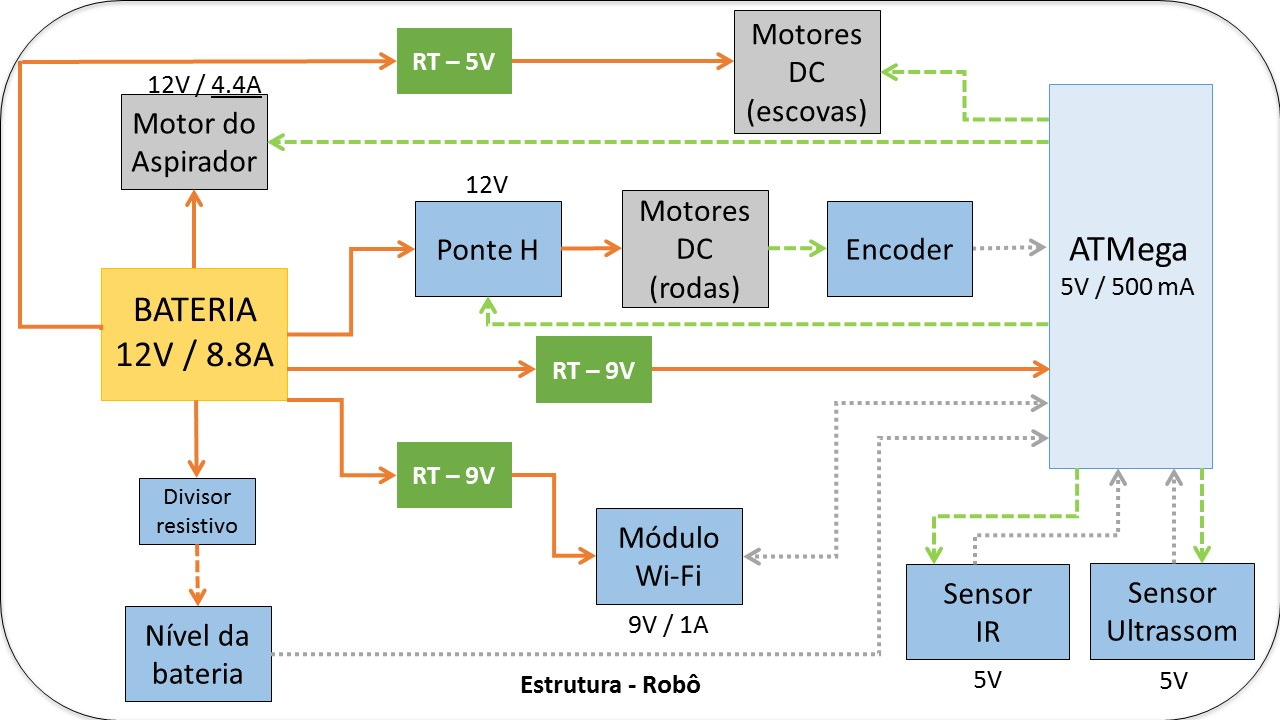
\includegraphics[scale=0.48]{figuras/plano_integracao_robo.jpg}               
   		\caption{Plano geral de integração dos subsistemas para o robô.}    
   		\label{img:integração_robô}                                            
   	\end{figure} 

   	\begin{figure}[H]                                                           
   		\centering                                                                
   		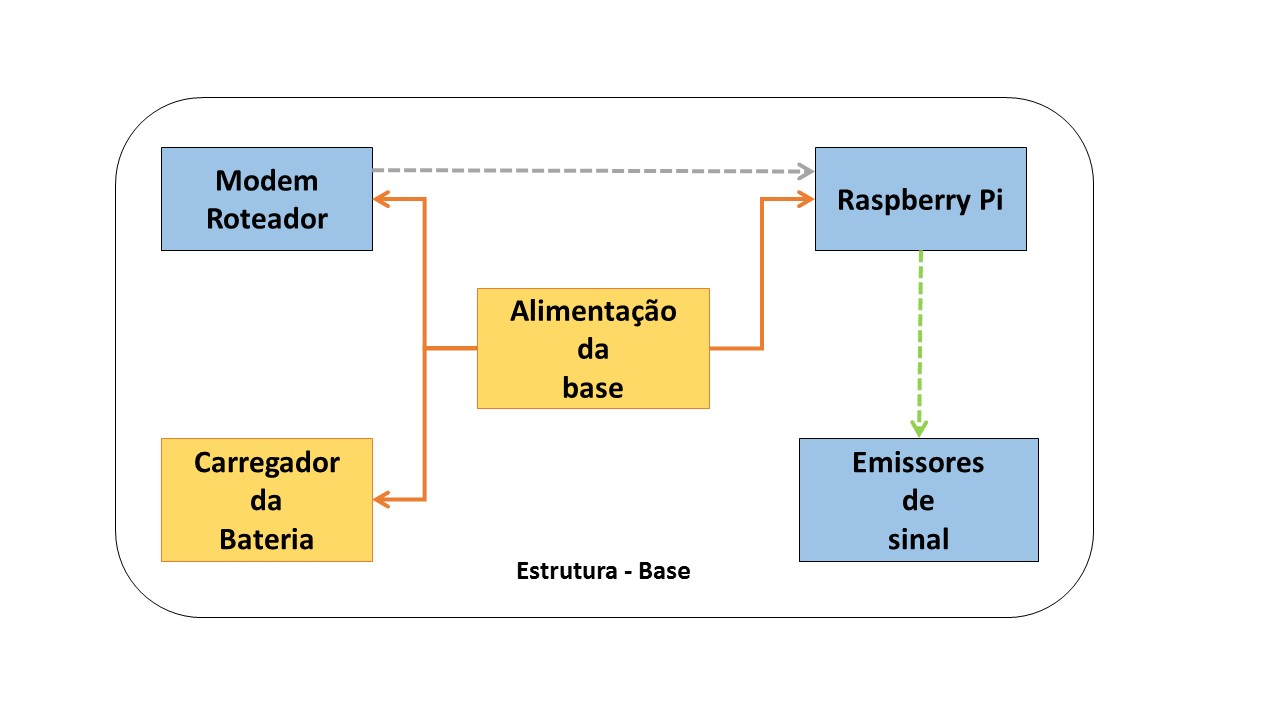
\includegraphics[scale=0.5]{figuras/plano_integracao_base.jpg}               
   		\caption{Plano geral de integração dos subsistemas para a base.}    
   		\label{img:integração_base}                                            
   	\end{figure} 

   	\noindent \textbf{Legenda}: \\
   	\noindent \textit{Setas de cor verde} - simbolizam que determinado bloco tem controle sobre um outro bloco. \\
   	\noindent \textit{Setas de cor laranja} - simbolizam a allimentação necessária para os componentes. \\
   	\noindent \textit{Setas de cor cinza} - simbolizam que há comunicação entre os blocos (os sentidos das setas indicam os caminhos dos dados).
% section plano_de_integração_e_validação (end)

\section{Testes de validação do plano de integração}
\label{sub:validação_plano_integração}
   \begin{itemize}
   		\item \textbf{Sistema de Sucção}

   			\begin{enumerate}
		      \item \textbf{Alimentar o aspirador com a bateria e testar a eficácia de aspiração de partículas}

		         O aspirador ao ser ligado a bateria obteve uma boa sucção, assim como nos testes de bancada utilizando a fonte de tensão. Entretanto, depois de alguns minutos ligados, a bateria começa a perder diferença de potencial, fazendo com que o aspirador comece a perder eficiência. Após 12 minutos, a bateria já não possuía tensão para manter o sistema funcionando de forma eficiente. Constatou-se também uma alta temperatura nas baterias. 

		         Outro teste realizado com as baterias escolhidas foi utilizando um regulador de tensão, para fornecer a potência necessária ao aspirador. Foi integrado o circuito regulador ao aspirador e ligado utilizando as baterias. O resultado foi positivo, verificando que elas forneciam 12 V, e o aspirador funcionando de modo esperado.

		      \item \textbf{Alimentar o motor escova e garantir que ele esteja rodando}

		         A alimentação foi suficiente para garantir a rotação do motor. Verificou-se que após um tempo grande de funcionamento, o temperatura do motor amolece a cola utilizada para sua fixação. Durante os testes com a escova, o motor DC utilizado teve um travamento repentino do eixo. Acredita-se que parte da sujeira entrou no motor, causando o seu travamento completo. 

		      \item \textbf{Testar os transistores do motor da escova e do aspirador}

		         Não foi possível realizar esse teste devido ao mal funcionamento das baterias. 

		      \item \textbf{Testar o sinal de controle do arduino até os transistores}

		         Não foi possível realizar esse teste devido ao mal funcionamento das baterias. 

		      \item \textbf{Ligar a aspiração e a escova com o sistema funcionando em 100\%}

		         Esse teste não foi realizado devido ao mal funcionamento que ocorreu nas novas baterias adquiridas. No dia do teste de integração, o aspirador conectado a um regulador de voltagem, para ajustar a tensão para 12 V funcionou individualmente. Mas ao conectar o aspirador ao resto do sistema e ligar os componentes do robô às baterias, nenhum componente do sistema ligou. Depois de analisar cuidadosamente para identificar o problema, constatou-se que a bateria não fornecia tensão nem corrente. Para resolver esse problema, foram adquiridas mais 3 baterias que serão destinadas para o uso exclusivo para a alimentação do sistema de sucção. 
		   \end{enumerate}

		\item \textbf{Estrutura do robô}

		Ao inicar a parte de integração dos subsistemas, a estrutura do robô apresentou problemas para se locomover conforme os comandos enviados a ele. De maneira geral, a equipe de estrutura identificou 3 principais problemas: 

		\begin{enumerate}
   			\item O suporte desenvolvido era largo e não estava tão justo as rodas, sendo que para compensar esta folga e melhorar o amortecimento tal espaço foi preenchido com borracha, porém com a adição do peso dos demais subsistemas a base as rodas acabaram por sair do alinhamento. Com isso o robô passou a não se mover mais em linha reta, e sim em círculos, o que ocasionaria vários problemas em outras áreas.

   			\item A posição das rodas, que foram fixadas inicialmente no centro da base, porém esse modelo não ofereceu a estabilidade necessária para a alocação dos subsistemas, além de dificultar a movimentação, que ocorreu também devido aos furos que não ficaram perfeitamente alinhados.

   			\item Originalmente não seriam utilizados encoders nas rodas, porém foi detectado que seriam necessários para melhorar o controle. Com isso o projeto original dos suportes das rodas e da base deveriam passar por algumas mudanças estruturais para poder adaptar tais componentes. O suporte feito originalmente não tinha os cortes necessários, então foi redesenhado para que pudesse ter, sem comprometer sua capacidade de fixação.


   		\end{enumerate}

   \end{itemize}
   

   \section{Modificações realizadas após os testes}
   \label{sub:mudanças}
   \begin{itemize}
      \item Troca do motor da escova:

         Devido ao travamento do motor da escova, foi necessário realizar a troca do mesmo. O novo motor DC colocado possui 9V de tensão nominal e 0.5 A de corrente nominal quando o eixo está carregado.

         \begin{figure}[H]                                                           
            \centering                                                                
            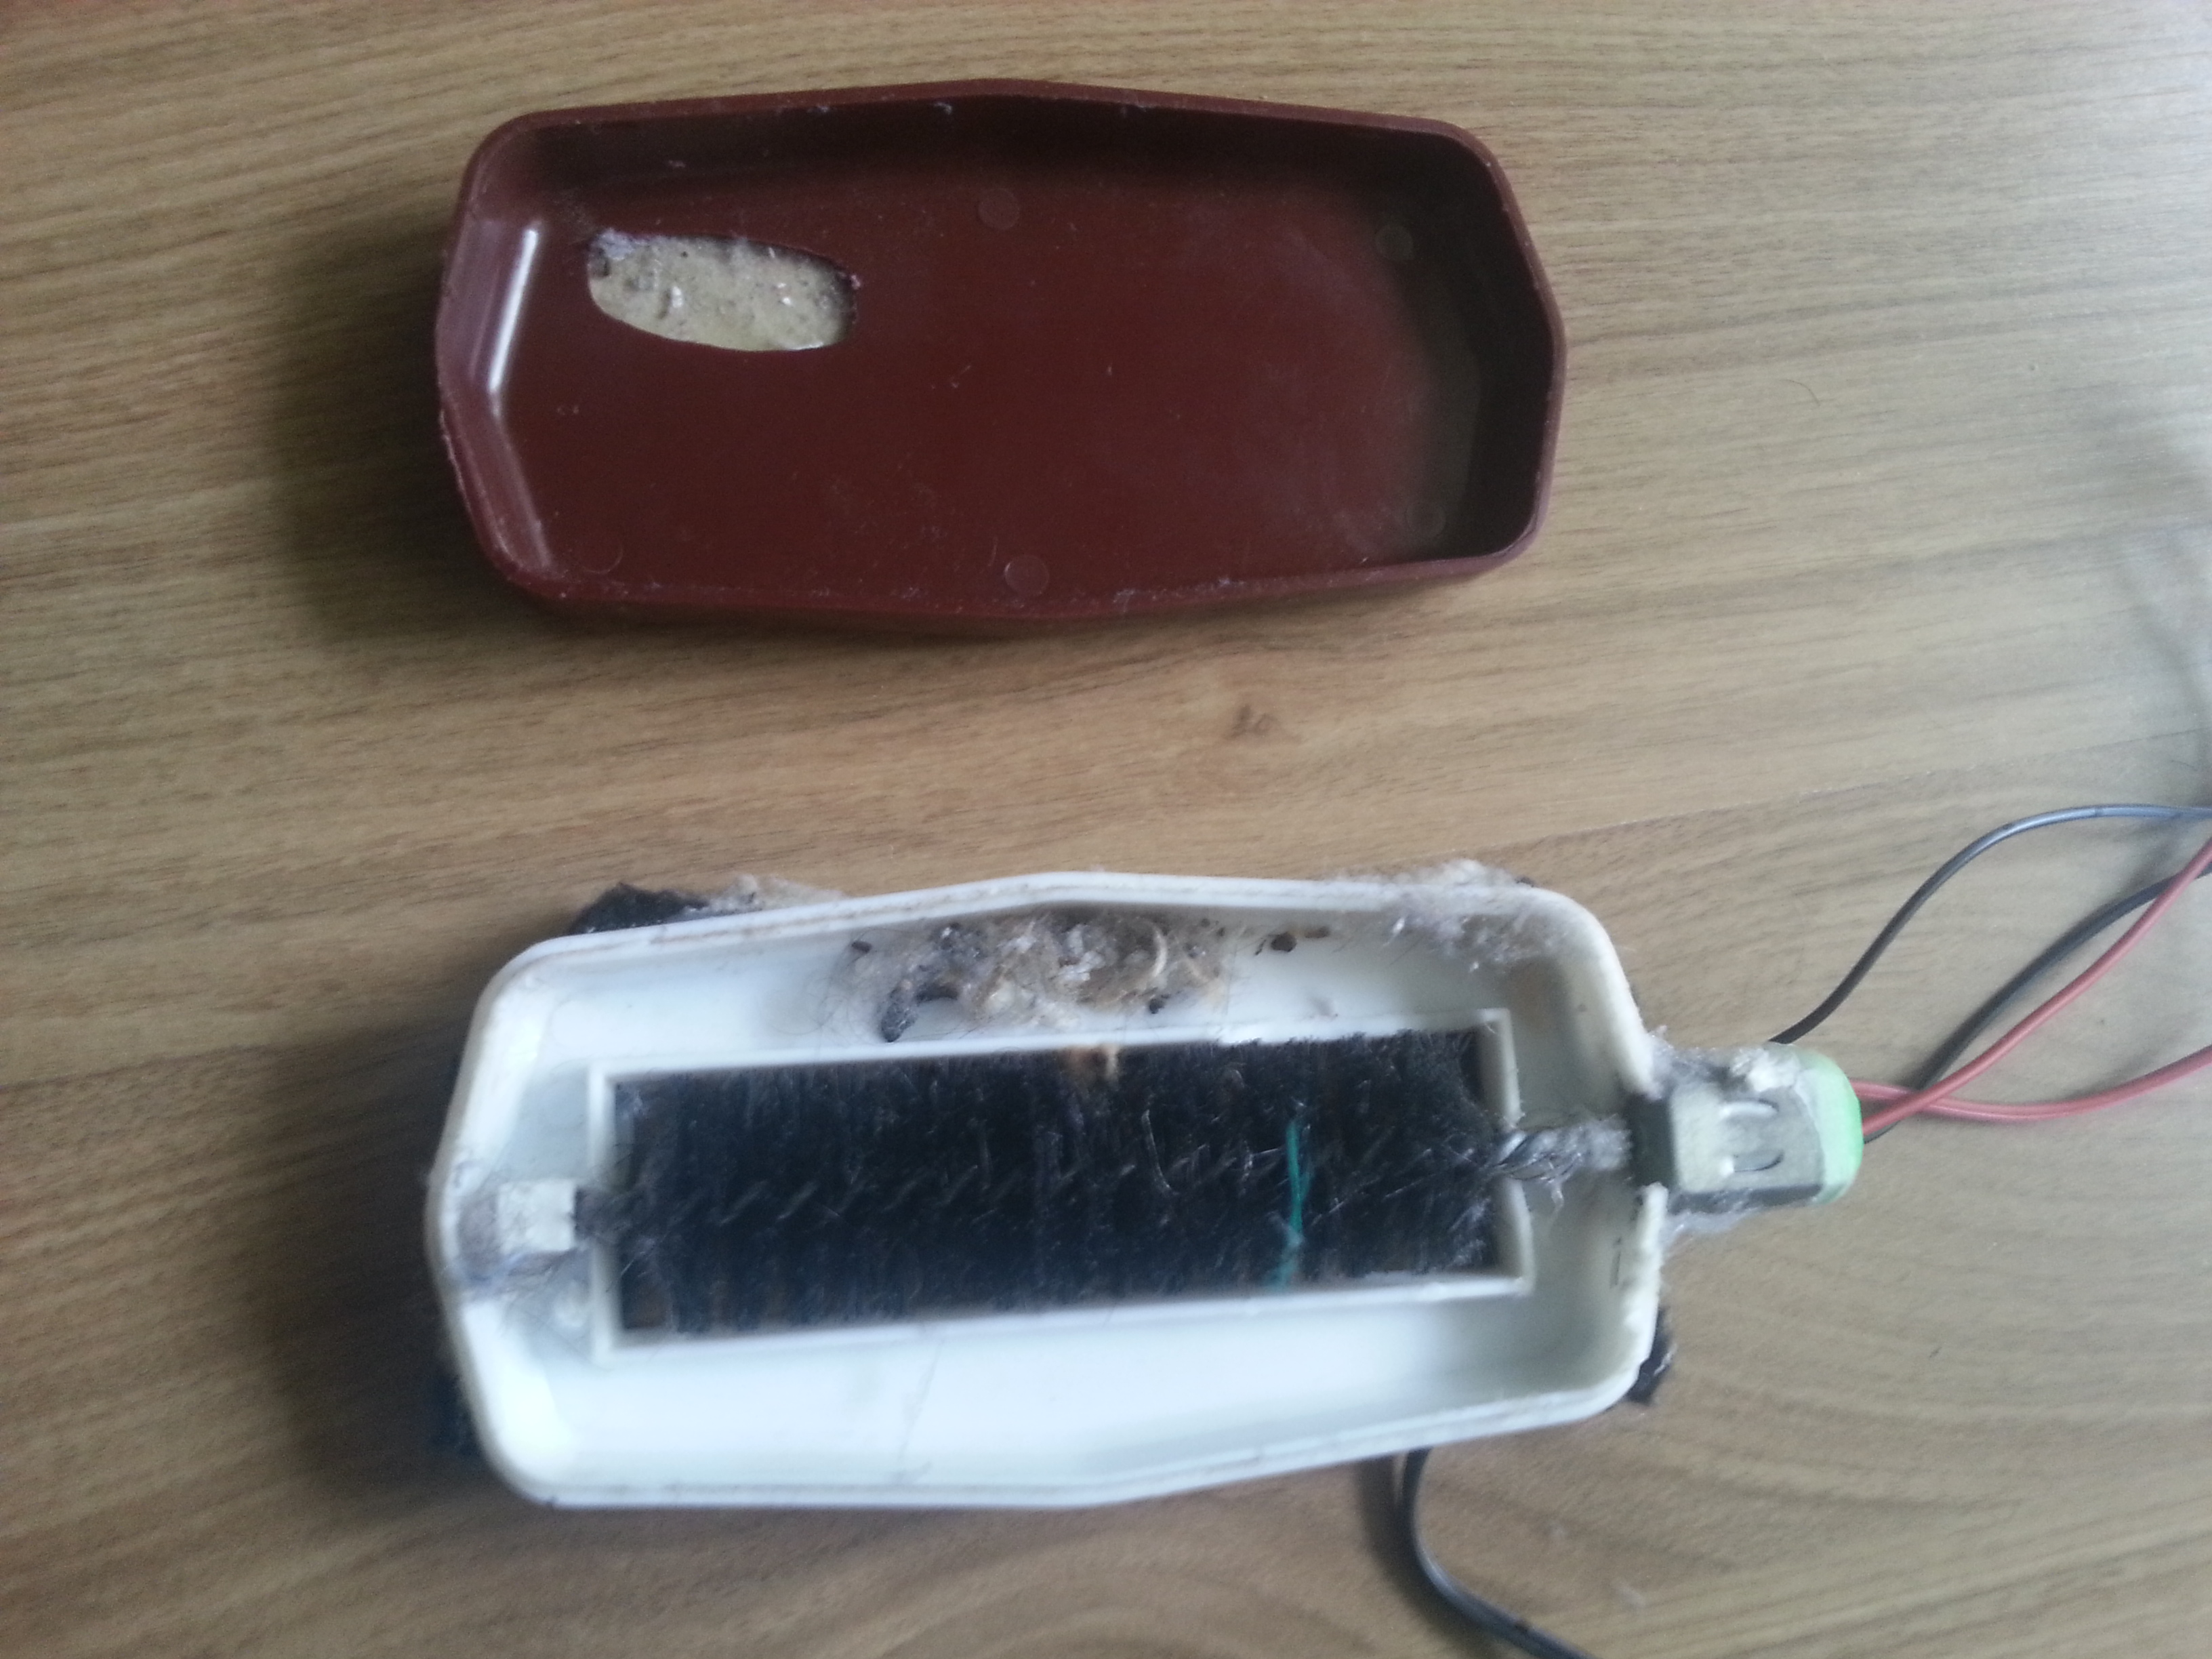
\includegraphics[scale=0.1]{figuras/SuccaoPC3_1.jpg}               
            \caption{Teste de coleta de sujeira com o novo motor acoplado.}    
            \label{img:teste_coleta}                                            
         \end{figure} 

      \item Troca dos cabos do aspirador e da escova:

         Foram adicionados cabos mais grossos e resistentes devido a quantidade de corrente que está sendo utilizada no circuito. 

      \item Acréscimo de mais pano na escova:

         Foi adicionado mais pano a escova com o objetivo de aumentar a eficiência do sistema de sucção. O pano adicionado garante que a sujeira seja varrida e contida ao alcance das cerdas da escova, de forma a garantir mais tempo para o sistema coletar a sujeira.

         \begin{figure}[H]                                                           
            \centering                                                                
            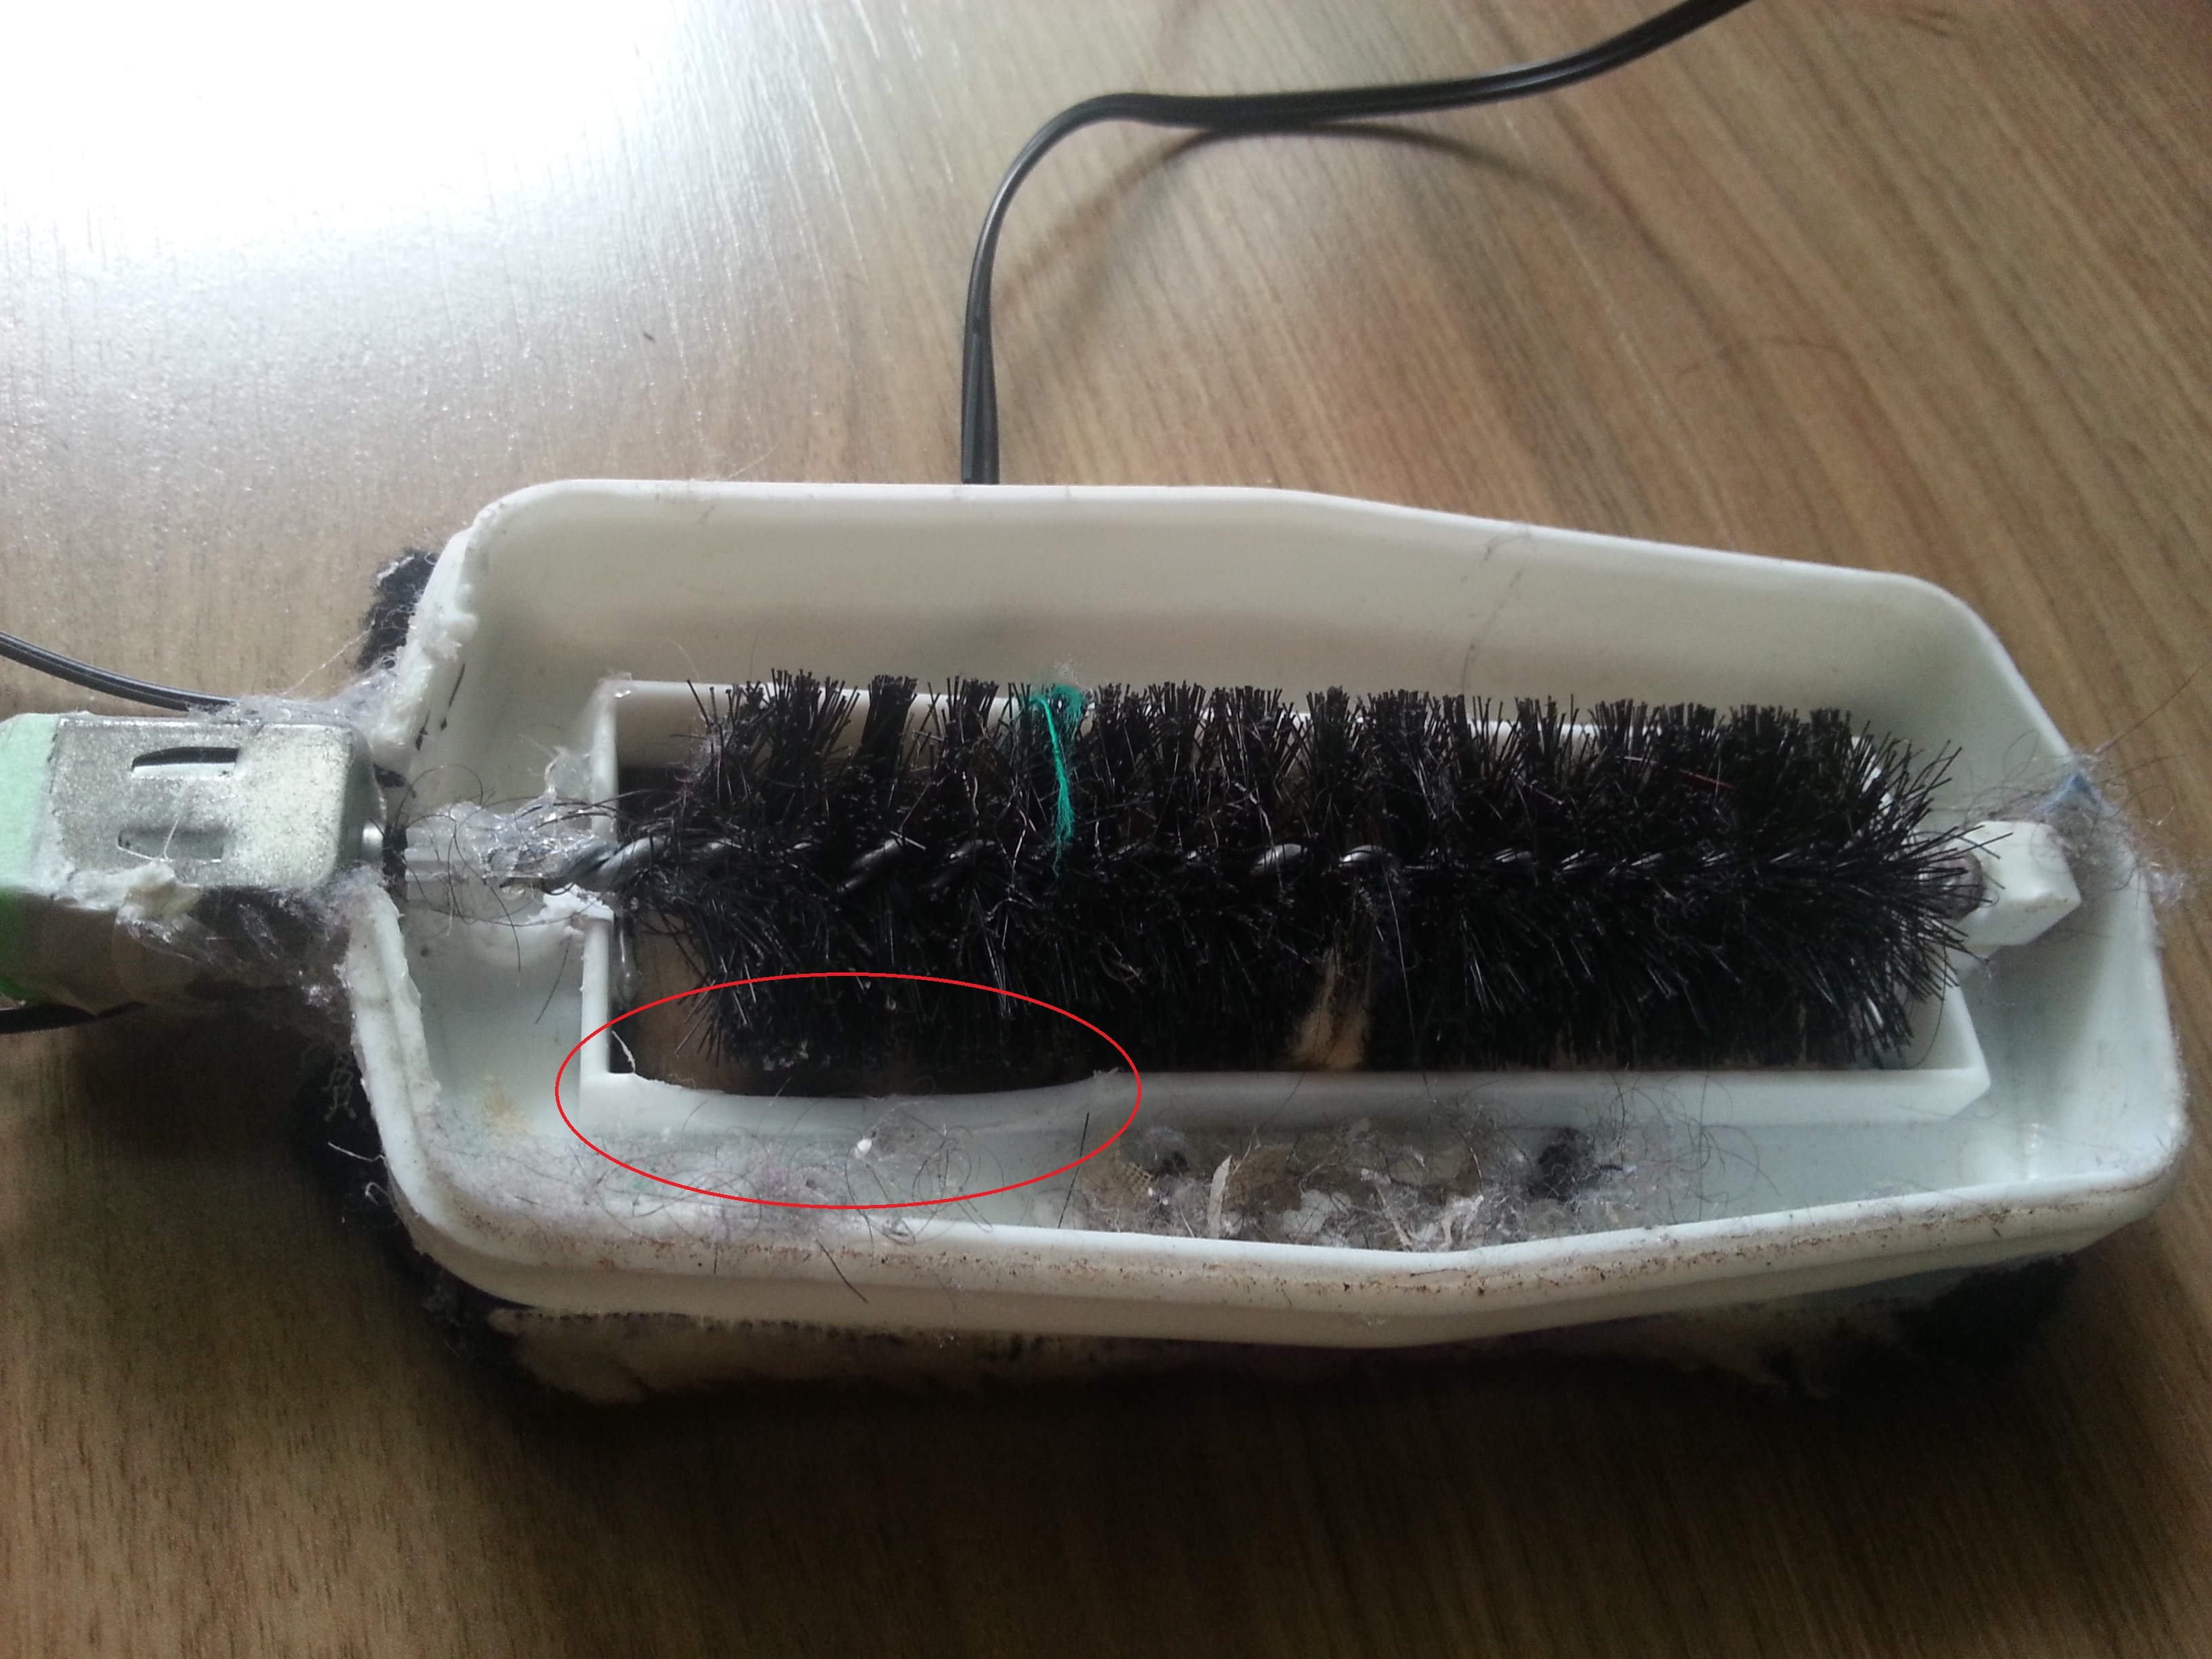
\includegraphics[scale=0.1]{figuras/SuccaoPC3_2.jpg}               
            \caption{Teste de coleta de sujeira após o acréscimo de pano a escova.}    
            \label{img:teste_coleta_pano}                                            
         \end{figure} 

      \item Modificação estrutural interna da escova

         Foi aberto um vão na parte interna da escova que fica próxima ao cano do aspirador. Essa modificação aumentou drasticamente a eficiência na coleta de sujeira por parte da escova.

         \begin{figure}[H]                                                           
            \centering                                                                
            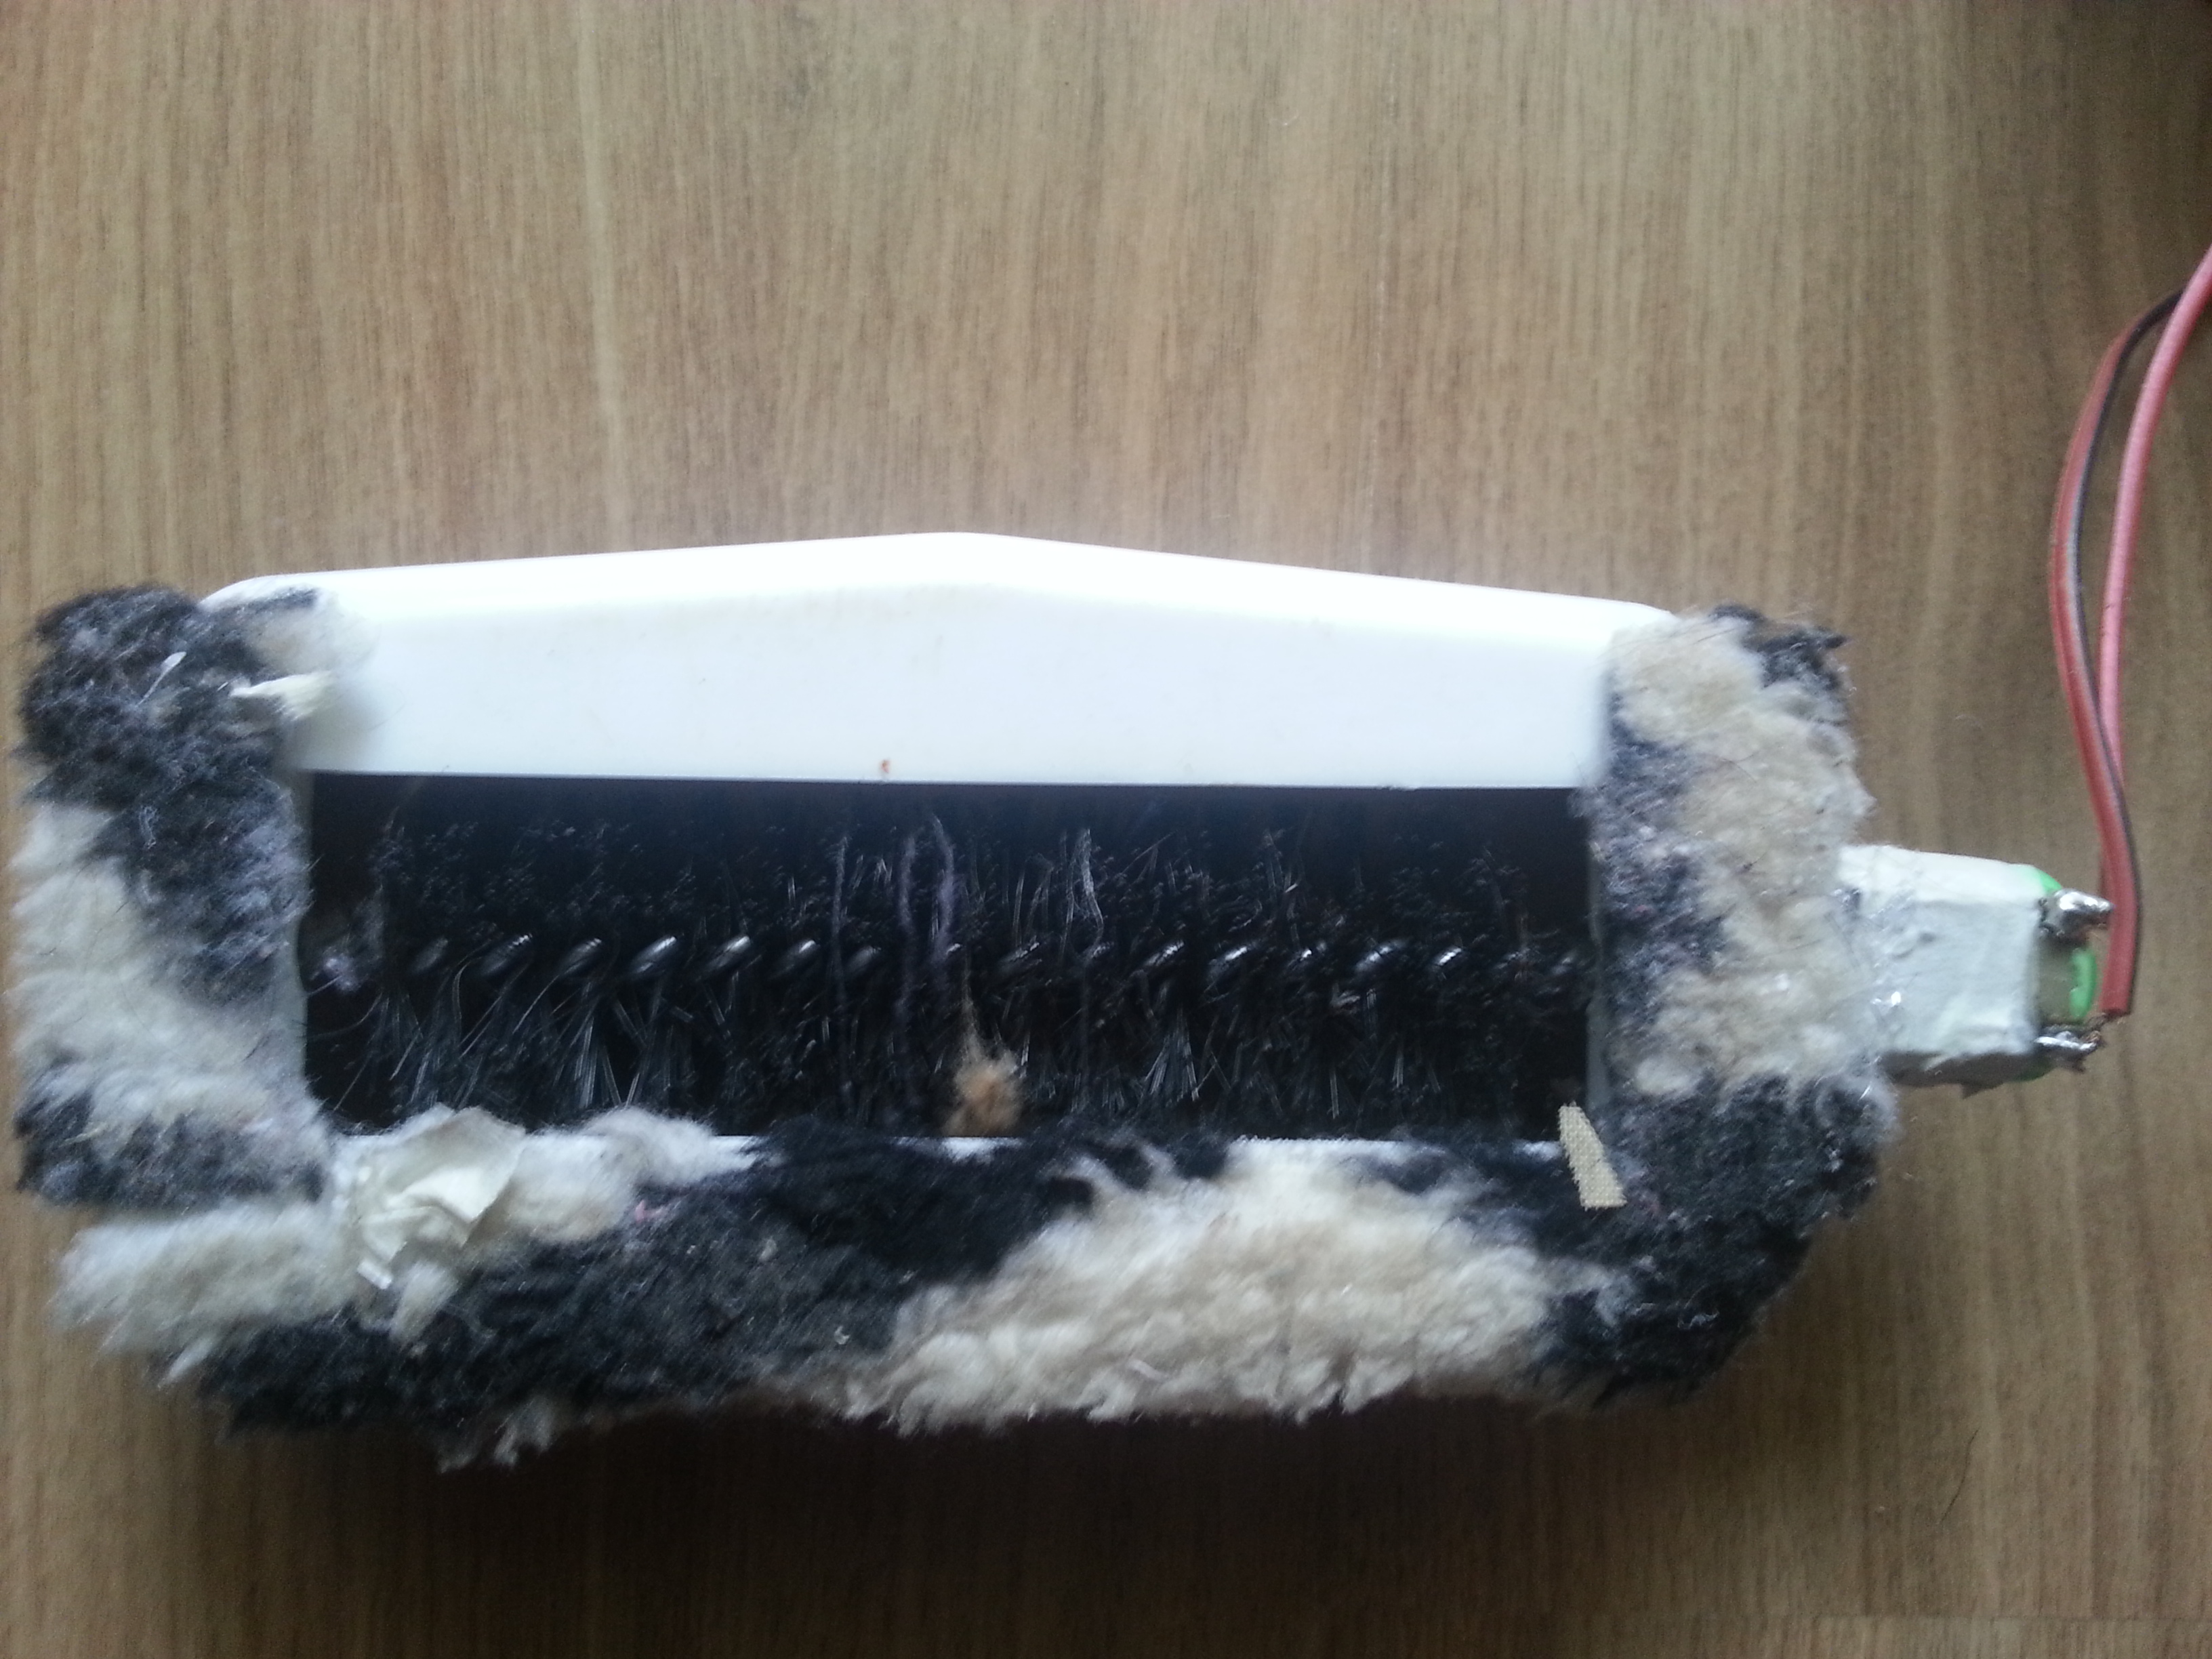
\includegraphics[scale=0.1]{figuras/SuccaoPC3_3.jpg}               
            \caption{Teste da coleta de sujeira com a abertura de parte da parede interna.}    
            \label{img:teste_coleta_sujeira}                                            
         \end{figure}

      \item Troca da mangueira do aspirador:

         A mangueira antiga utilizada no aspirador era sanfonada, o que prejudica o desempenho do aspirador. Foi adicionada uma mangueira de borracha com superfície interna lisa, com o objetivo de diminuir a perda de carga do sistema.  

         \begin{figure}[H]                                                           
            \centering                                                                
            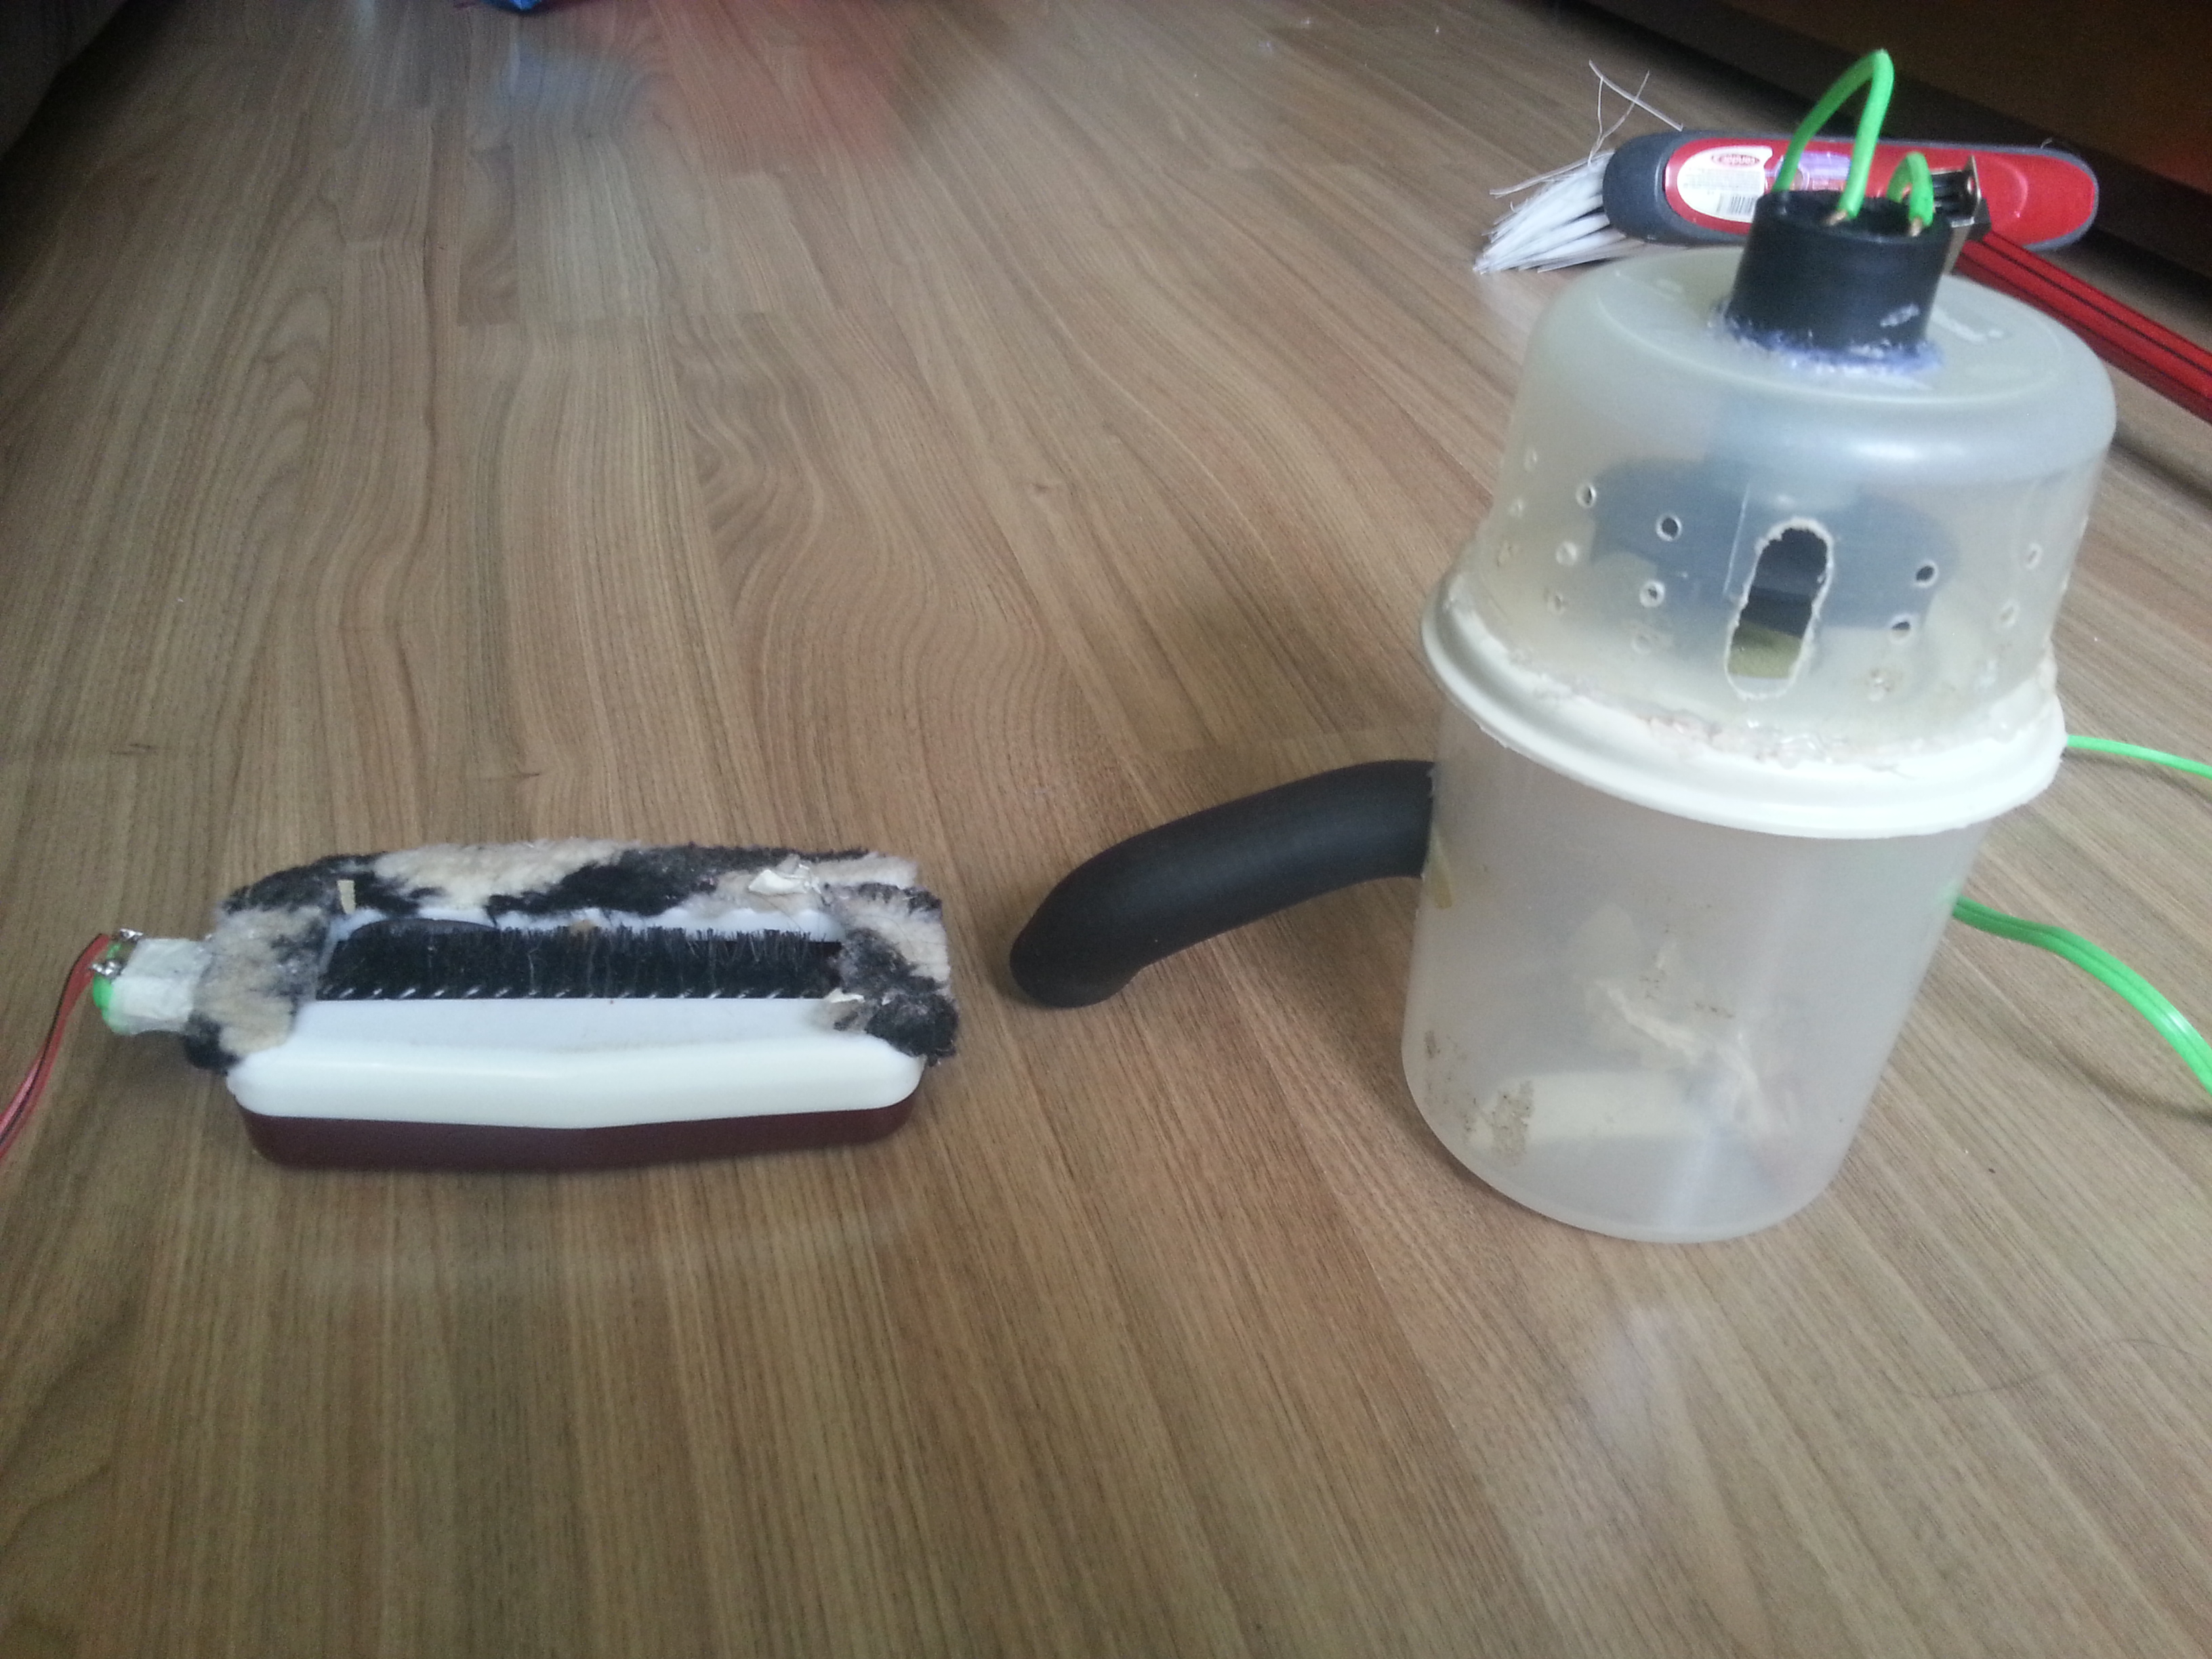
\includegraphics[scale=0.1]{figuras/SuccaoPC3_4.jpg}               
            \caption{Imagem dos novos cabos e da nova mangueira ligada ao aspirador.}    
            \label{img:novo_sistema_sucção}                                            
         \end{figure}

      \item Adaptação do suporte das rodas:

      	Para solucionar este problema, uma adaptação ao suporte foi feita para que as rodas não ficassem tão folgadas na estrutura, garantindo que não ficassem desalinhadas quando sujeitas a carga. Abaixo temos a comparação do primeiro suporte com o adaptado, que se mostrou muito mais eficiente nos testes:

   			(Inserir figuras e fazer a referencia acima)

   	  \item Posicionamento das rodas:

   	  	Para solucionar este problema, uma nova posição para as rodas foi definida de modo que esta pudesse oferecer uma estabilidade melhor, consequentemente aguentando uma distribuição mais uniforme de peso. As rodas foram deslocadas um pouco, não ficando mais no centro, mas na parte traseira da base, o antes e depois das modificações pode ser visto nas imagens abaixo:

   			(Inserir figuras e fazer a referencia)

   	  \item Adição dos encoders na estrutura:


   		Feitos os furos constatou-se que o eixo que seria fixado o encoder deveria ser alongado, caso contrário não seria possível a adaptação. Para alongar o eixo, foram utilizados raios de bicicleta, que foram parafusados ao eixo e tiveram o encoder preso em sua ponta com massa plástica, garantindo uma fixação segura. Os sensores foram presos a base com parafusos. Pode-se observar os resultados da adaptação nas imagens a seguir:

   			(Inserir figuras e fazer as referencias)

   \end{itemize}
 		

% section plano_de_integração_e_validação (end)